%THIS CODE IS MY OWN WORK, IT WAS WRITTEN WITHOUT CONSULTINGA TUTOR OR CODE WRITTEN BY OTHER STUDENTS - Jae Kyum Kim
\documentclass{article}
\usepackage{pythonhighlight}
\usepackage{graphicx}
\usepackage{subcaption}

\title{CS470 Homework 3}
\date{2020-02-27}
\author{Jaekyum Kim}

\begin{document}

  \pagenumbering{gobble}
  \maketitle
  \newpage
  \pagenumbering{arabic}
\paragraph{Collaboration Statement}
THIS CODE IS MY OWN WORK, IT WAS WRITTEN WITHOUT CONSULTING A TUTOR OR CODE WRITTEN BY OTHER STUDENTS - Jaekyum Kim

\section{Introduction}
The program is executable with 3 parameters: the name of the input dataset file, the value of K, and the name of the output file. The two kinds of dataset I used in this project was "iris.data" and "wine.data". The output contains numerical class labels (formatted as one number per row) for all the records in the test dataset and reports the sum squared error (SSE) and silhouette coefficient in the last row. 

\section{Cluster Initialization}
A conventional K-means algorithm first arbitrarily chooses whatever a user input's K is and randomly chooses K-number of clusters among the dataset. The code to choose K-number of datapoint is following (this function was commented out in the code):
\begin{python}
for i in range(0,k):
    index = random.randrange(0, len(dataset), 3)
    initialization.append(dataset[index])
\end{python}
However randomly choosing initialization points for clusters can possibly cause a problem later when the algorithm finishes. While experimenting this issue, I have noticed that this naive approach can produce a negative Silhouette coefficient. According to the textbook on the section of coefficient points, when the silhouette coefficient value is negative (i.e., b(o) < a(o)), this means that, in expectation, o is closer to the objects in another cluster than to the objects in the same cluster as o. 
In many cases, this is a bad situation and should be avoided. Therefore to fix the problem, I have implemented the algorithm to pick K-number of farthest point within each other, so the K-means algorithm is guaranteed to find the most optimal cluster points before running the iteration. Because the algorithm chooses fixed K-number of points, the silhouette point will never hit the negative number. The code for farthest point initialization is the following: 
\begin{python}
def spitDist(firstcentroid, my_list):
    distDict.clear()
    
    for eachline in dataset:
        difference = map(operator.sub, firstcentroid, eachline)
        squared = [i ** 2 for i in difference]
        listsummed = sum(squared)
        euclidean = math.sqrt(listsummed)
    
        #print("calculating distance between: ",eachline,"and",firstcentroid)
        #print("calculated euclidean for this edge: ", euclidean)
        
        eachline = tuple(eachline)
        if eachline not in initialization:
            distDict[tuple(eachline)] = euclidean #node that is farthest out
            maxlength = euclidean
        
    return distDict

if k >= 2:
    for eachcluster in initialization:
        tmp=spitDist(eachcluster, my_list)
        a = sorted(tmp.items(), key=lambda x: x[1],reverse=True)
            
        candidateslist = []
            
        for eachvector in a:
            candidateslist.append(eachvector[0])#make list of candidates in sorted order
            
        if len(initialization) != 1:
            ans = []
            for eachItemI in candidateslist:
                for eachItemJ in result:
                    if eachItemI == eachItemJ:
                        ans.append(eachItemI)
            result = list(ans)

            initialization.append(ans[0])
        elif len(initialization) == 1:
            initialization.append(candidateslist[0])
            result = list(candidateslist)

        if(len(initialization) == k):
            break
\end{python}
To briefly explain the algorithm for farthest point cluster selection, The algorithm first choose a random first point to begin with because you need a point to start measuring points that are farthest away from each other.  This routine would have been easy if there was a built in collection for sets that keep order, then first i could just find a set of distance from a chosen cluster point to every other points and get the point that are farthest away. Then, I intersect those two sets of sorted distance to find the common longest distance. If I keep running the routine, then I would be able to find K-number of cluster points that are farthest away from each other. 
    \newpage

\section{Elbow method}

\begin{figure}[h!]
  \centering
  \begin{subfigure}[b]{.6\linewidth}
    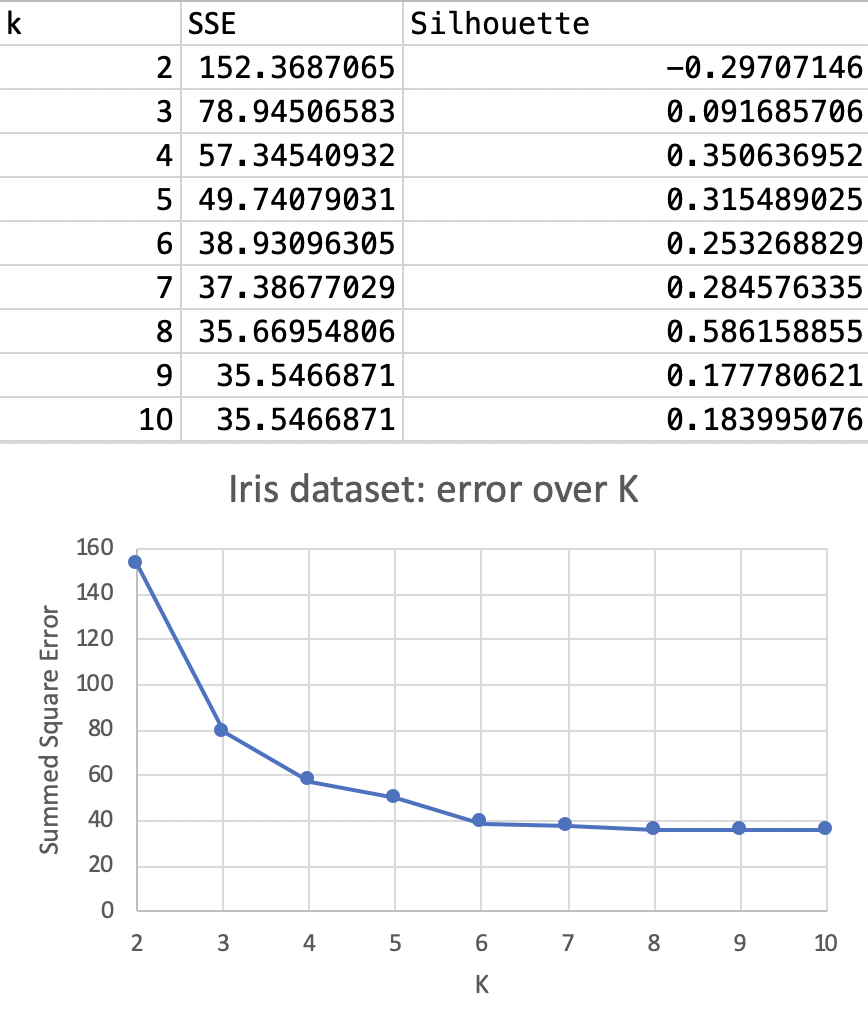
\includegraphics[width=\linewidth]{one.jpg}
  \end{subfigure}
  \caption{SSE vs K for Iris dataset }

  \end{figure}
      \paragraph{Figure 1}
As shown in the dataset, only three types of Iris species occur. The relationship graphed displays that the desirable K is in between 2 and 4. The bend in the trendline is at k=3.
    \newpage

\begin{figure}[h!]
  \centering
  \begin{subfigure}[b]{.6\linewidth}
    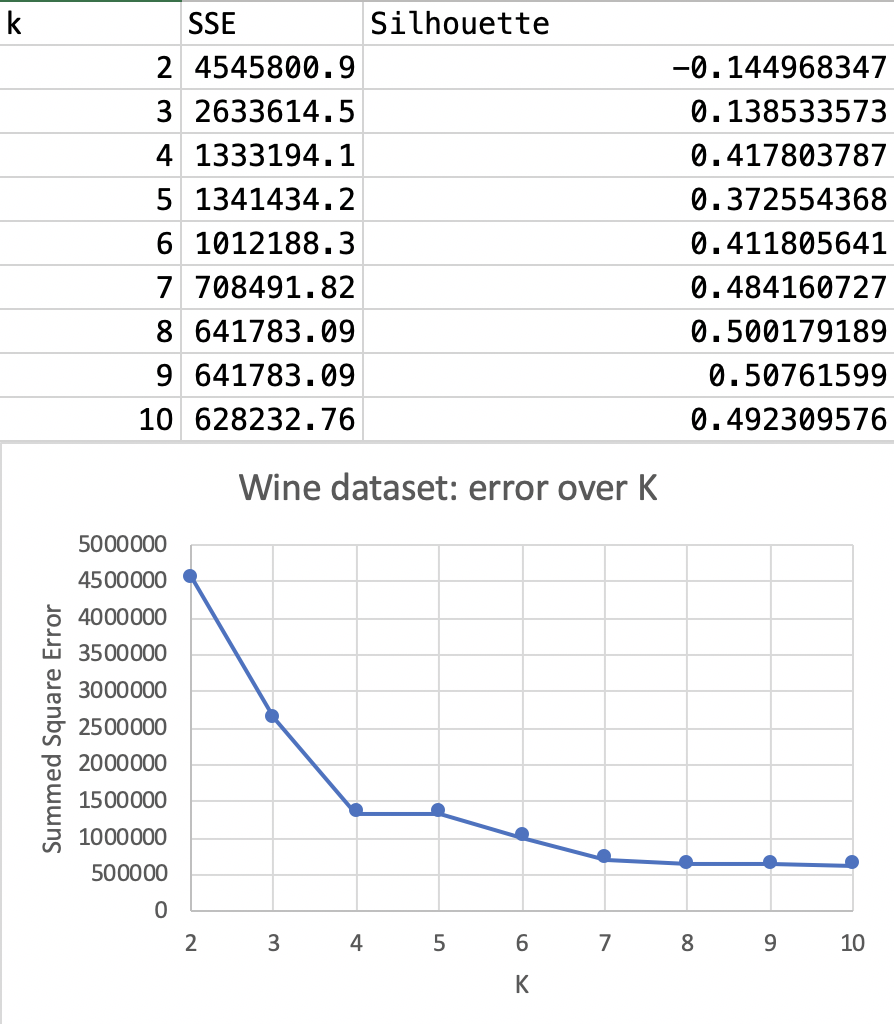
\includegraphics[width=\linewidth]{two.jpg}
  \end{subfigure}
  \caption{SSE vs K for Wine dataset }

  \end{figure}
        \paragraph{Figure 2}

    As shown in the dataset, only three types of wine variations can occur. The relationship graphed displays that the desirable K is in between 2 and 4. The bend in the trendline is at k=3.

\end{document}



